\chapter{푸아송 괄호, 생성자, 각운동량}

\lectureoverview{푸아송 괄호는 해밀턴 방정식을 간결하게 다시 쓰는 방법에 그치지 않는다. 변환을 생성하는 대수적 연산이다. 해밀토니안과의 푸아송 괄호는 시간 변화를 생성하고, 운동량과의 푸아송 괄호는 병진을 생성하며, 각운동량과의 푸아송 괄호는 회전을 생성한다. 이 관점에서 대칭성과 보존은 하나의 푸아송 괄호가 영이 되는 현상을 서로 다르게 해석한 것이다. 조화 진동자에서 이 생각을 전개한 뒤, 오일러각을 도입하지 않고 각운동량 대수를 이용해 자이로스코프의 세차 운동을 구하겠다.}

\section{해밀턴 궤적을 따라 변하는 함수}

위상 공간에서 충분히 미분 가능한 함수 \[
  F=F(q_1,\ldots,q_n,p_1,\ldots,p_n)
\]를 생각하자. 이 함수는 두 가지 방식으로 볼 수 있다. 첫째, 위상 공간의 모든 점에 수를 하나 대응시킨다. 둘째, 해밀턴 궤적을 하나 정하면 점 \((q(t),p(t))\)가 움직이므로 시간의 함수가 된다. 그 궤적을 따라가면 \begin{equation}
  \frac{dF}{dt}
  =
  \sum_i\left(
    \frac{\partial F}{\partial q_i}\dot q_i
    +\frac{\partial F}{\partial p_i}\dot p_i
  \right).
  \label{eq:l8-chain-rule}
\end{equation} 해밀턴 방정식 \begin{equation}
  \dot q_i=\frac{\partial H}{\partial p_i},
  \qquad
  \dot p_i=-\frac{\partial H}{\partial q_i},
  \label{eq:l8-hamilton-equations}
\end{equation}을 대입하여 다음을 얻는다. \begin{equation}
  \frac{dF}{dt}
  =
  \sum_i\left(
    \frac{\partial F}{\partial q_i}
    \frac{\partial H}{\partial p_i}
    -
    \frac{\partial F}{\partial p_i}
    \frac{\partial H}{\partial q_i}
  \right).
  \label{eq:l8-fdot-expanded}
\end{equation} 오른쪽에 있는 이 조합은 두 항 가운데 어느 것도 해밀토니안이 아닌 경우에도 고전역학 전반에 걸쳐 나타난다. 이에 따라 다음과 같이 정의한다. \begin{equation}
  \boxed{
  \{F,G\}
  =
  \sum_i\left(
    \frac{\partial F}{\partial q_i}
    \frac{\partial G}{\partial p_i}
    -
    \frac{\partial F}{\partial p_i}
    \frac{\partial G}{\partial q_i}
  \right).}
  \label{eq:l8-poisson-definition}
\end{equation} 따라서 식 ~\eqref{eq:l8-fdot-expanded}은 다음과 같다. \begin{equation}
  \boxed{\dot F=\{F,H\}.}
  \label{eq:l8-time-generator}
\end{equation}

\begin{classroomqa} \audiencequestion{두 번째 항을 \(H\)에서 임의의 함수 \(G\)로 바꾸어도 괄호가 여전히 \(F\)의 시간 미분인가요? \lecturetimestamp{00:05:45--00:06:15}} \lecturerresponse{아니다. 표기법을 일반화하는 중에 청중이 중요한 점을 짚었다. 식 ~\eqref{eq:l8-poisson-definition}은 위상 공간의 임의의 두 함수에 대해 \(\{F,G\}\)를 정의하지만, \(\dot F=\{F,G\}\)은 \(G\)가 해밀토니안일 때만 성립한다. 일반적인 \(G\)는 다른 무한소 변환을 생성한다.}\end{classroomqa}

시간의 작은 변화를 다음과 같이 쓰면 편리하다. \begin{equation}
  \delta_t F=\epsilon\,\{F,H\}.
  \label{eq:l8-small-time-step}
\end{equation} 이 형태는 뒤에서 다룰 내용을 미리 보여 준다. 시간 변화는 푸아송 괄호로 생성되는 더 큰 변환 계열의 한 구성원이다.

\section{괄호 대수}

이제 괄호를 그 자체의 미적분으로 다룰 수 있다. 그 규칙은 보통의 미분에서 나온다. \begin{align}
  \{A,B\}&=-\{B,A\}, \label{eq:l8-antisymmetry}\\
  \{A+B,C\}&=\{A,C\}+\{B,C\}, \label{eq:l8-additivity}\\
  \{\lambda A,B\}&=\lambda\{A,B\},
    \quad \lambda\ \text{constant}, \label{eq:l8-scalar-rule}\\
  \{AB,C\}&=A\{B,C\}+\{A,C\}B. \label{eq:l8-leibniz}
\end{align} 이 네 줄은 각각 반대칭성, 가법성, 상수배에 대한 선형성, 라이프니츠 법칙을 나타낸다. 고전적 위상 공간 함수의 곱셈은 가환적이므로 마지막 줄에서 보통의 인수 \(A\)와 \(B\)의 위치는 중요하지 않다. 양자역학의 연산자에서는 더 이상 그렇지 않다. 반대칭성은 또한 다음을 함의한다. \begin{equation}
  \{A,A\}=0.
  \label{eq:l8-self-bracket}
\end{equation}

정준 좌표의 기본 푸아송 괄호는 다음과 같다.
\begin{equation}
  \boxed{
  \{q_i,q_j\}=0,\qquad
  \{p_i,p_j\}=0,\qquad
  \{q_i,p_j\}=\delta_{ij}.}
  \label{eq:l8-canonical-brackets}
\end{equation}
\(q_i\)에만 의존하는 함수는 \(q_i\)에만 의존하는 다른 함수와 푸아송 괄호가 영이다. \(p_i\)에만 의존하는 함수들에도 같은 성질이 성립한다. 푸아송 괄호가 영이 아니려면 정준 좌표와 그 켤레 운동량이 짝을 이루어야 한다. 식~\eqref{eq:l8-canonical-brackets}의 크로네커 델타는 지표가 서로 일치하는 경우에만 짝을 이룬다는 것을 나타낸다.

\subsection{조화진동자로 살펴보기}

다음을 생각하자. \begin{equation}
  H=\frac{p^2}{2m}+\frac{kq^2}{2}.
  \label{eq:l8-oscillator-hamiltonian}
\end{equation} 이제 괄호의 규칙과 식 ~\eqref{eq:l8-time-generator}만을 의도적으로 사용하겠다. 먼저, \begin{align}
  \dot q
  &=\{q,H\}\\
  &=\frac{1}{2m}\{q,p^2\}\\
  &=\frac{1}{2m}\left(p\{q,p\}+\{q,p\}p\right)\\
  &=\frac{p}{m}.
  \label{eq:l8-qdot-oscillator}
\end{align} 퍼텐셜 항은 \(\{q,q^2\}=0\)이므로 사라진다. 마찬가지로, \begin{align}
  \dot p
  &=\{p,H\}\\
  &=\frac{k}{2}\{p,q^2\}\\
  &=\frac{k}{2}\left(q\{p,q\}+\{p,q\}q\right)\\
  &=-kq.
  \label{eq:l8-pdot-oscillator}
\end{align} 여기서 음의 부호는 반대칭성 \(\{p,q\}=-\{q,p\}=-1\)에서 바로 나온다. 이 두 일차 방정식을 결합하면 다음을 얻는다. \begin{equation}
  m\ddot q=-kq.
  \label{eq:l8-hooke-equation}
\end{equation}

\begin{figure}[htbp]\centering
  
\includegraphics[width=0.82\textwidth]{lecture_08_figure_01.png}\caption{조화진동자 해밀토니안과 \(\dot q=p/m\) 및 \(\dot p=-kq\)을 얻는 두 푸아송 괄호 계산.}\lectureframe{00:23:20}\end{figure}

계산 도중, 강의실에서는 \emph{푸아송 괄호를 취하다}에 해당하는 동사를 찾다가 잠정적으로 \emph{푸아송화하다}를 쓰기로 한다. 이 농담은 관점의 실질적인 변화를 나타낸다. 대수를 알고 나면 정의에서 매번 결과를 다시 유도하지 않고 대수 자체를 바로 사용할 수 있다.

\begin{classroomqa}\audiencequestion{이 수학적 구조는 군인가요, 대수인가요? 역원이 있나요? \lecturetimestamp{00:23:48--00:24:16}} \lecturerresponse{군은 아니다. 괄호 연산은 군에 필요한 항등원과 역원을 제공하지 않는다. 위상 공간 함수들은 푸아송 대수를 이룬다. 보통의 가환적 곱셈과 덧셈에 더해, 반대칭 괄호가 있고 라이프니츠 법칙을 만족한다. 통상적인 추상적 정의를 완성하려면 야코비 항등식도 필요하지만, 이 강의에서는 다루지 않는다.}\end{classroomqa}

\begin{classroomqa}\audiencequestion{푸아송 괄호와 양자 교환자의 관계는 무엇인가요? \lecturetimestamp{00:24:18--00:25:00}} \lecturerresponse{강의에서는 미리보기만 제시한다. 양자역학으로 넘어갈 때 고전적 괄호는 개략적으로 다음과 같이 바뀐다. \[
    \{A,B\}_{\mathrm{PB}}
    \longleftrightarrow
    \frac{1}{i\hbar}[\widehat A,\widehat B].
  \] 이 대응에는 연산자 순서와 양자화에 관한 단서가 필요하며, 여기서는 정리로 사용하지 않는다.}\end{classroomqa}

조화진동자의 경우 괄호는 해밀턴 방정식을 다시 얻는 데 그쳤다. 괄호의 생성자가 \(H\) 이외의 보존량일 때 그 진가가 드러난다.

\section{회전 대칭성에서 각운동량 얻기}

강의 앞부분에서 다룬 뇌터 구성의 무한소 형태를 떠올려 보자. 연속 대칭에 의해 좌표가 \begin{equation}
  \delta q_i=\epsilon F_i(q),
  \label{eq:l8-noether-variation}
\end{equation}만큼 변한다면, 여기서 고려하는 경우 그 보존량은 \begin{equation}
  G=\sum_i p_iF_i(q).
  \label{eq:l8-noether-charge}
\end{equation}이다. 전체 인자 \(\epsilon\)는 생략해도 된다. 보존량에 고정된 수를 곱해도 보존 법칙은 바뀌지 않는다.

입자 하나를 \(z\)축 둘레로 무한소 회전시키자. 강의에서 사용한 방향 규약에 따르면, \begin{equation}
  \delta x=-\epsilon y,\qquad
  \delta y=\epsilon x,\qquad
  \delta z=0.
  \label{eq:l8-z-rotation}
\end{equation} 식 ~\eqref{eq:l8-noether-charge}을 적용하면 다음과 같다. \begin{equation}
  L_z=-p_xy+p_yx=xp_y-yp_x.
  \label{eq:l8-lz}
\end{equation} \(x\), \(y\), \(z\)을 순환적으로 바꾸면, \begin{equation}
  \boxed{\begin{aligned}
    L_x&=yp_z-zp_y,\\
    L_y&=zp_x-xp_z,\\
    L_z&=xp_y-yp_x.
  \end{aligned}}
  \label{eq:l8-angular-components}
\end{equation} 이는 다음의 성분이다. \begin{equation}
  \boldsymbol L=\boldsymbol r\times\boldsymbol p.
  \label{eq:l8-cross-product}
\end{equation}

\begin{figure}[htbp]\centering
  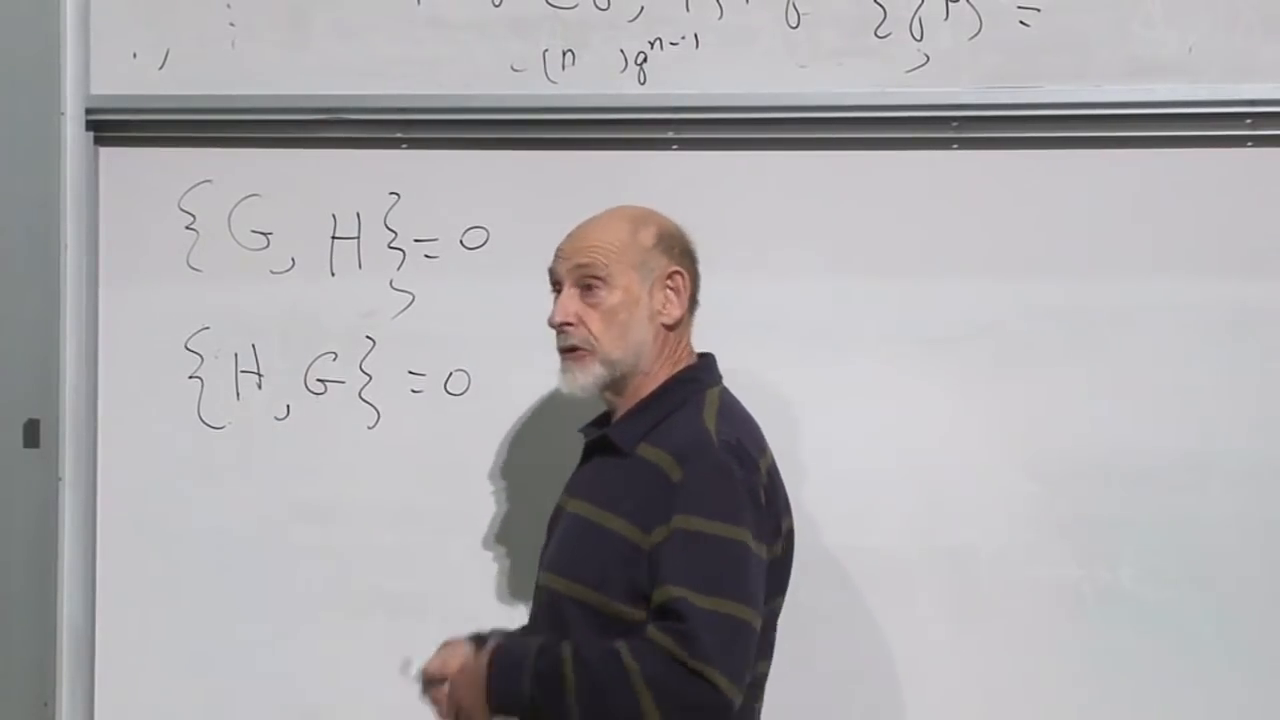
\includegraphics[width=0.82\textwidth]{lecture_08_figure_02.png}\caption{각운동량의 세 데카르트 성분과 이를 간결하게 나타낸 벡터곱 표현.}\lectureframe{00:34:00}\end{figure}

임의의 단위벡터 \(\boldsymbol n\)를 축으로 하는 회전은 \begin{equation}
  L_{\boldsymbol n}=\boldsymbol n\cdot\boldsymbol L.
  \label{eq:l8-arbitrary-axis}
\end{equation}에 의해 생성된다. 고립된 회전 대칭계에서는 세 성분이 모두 보존된다. 한 축 둘레의 회전만 대칭으로 남는다면, 그 축 방향 성분만 보존된다고 보장된다.

\section{각운동량은 회전을 생성한다}

회전 동역학 문제를 곧바로 풀기보다, 먼저 괄호를 취했을 때 \(L_z\)가 어떻게 작용하는지 살펴보자. 식 ~\eqref{eq:l8-lz}을 사용하면, \begin{align}
  \{x,L_z\}
  &=\{x,xp_y-yp_x\}
   =-y\{x,p_x\}
   =-y,\\
  \{y,L_z\}
  &=\{y,xp_y-yp_x\}
   =x\{y,p_y\}
   =x,\\
  \{z,L_z\}&=0.
  \label{eq:l8-position-rotation-brackets}
\end{align} 이는 식 ~\eqref{eq:l8-z-rotation}에 있는 계수와 정확히 일치한다.

\begin{figure}[htbp]\centering
  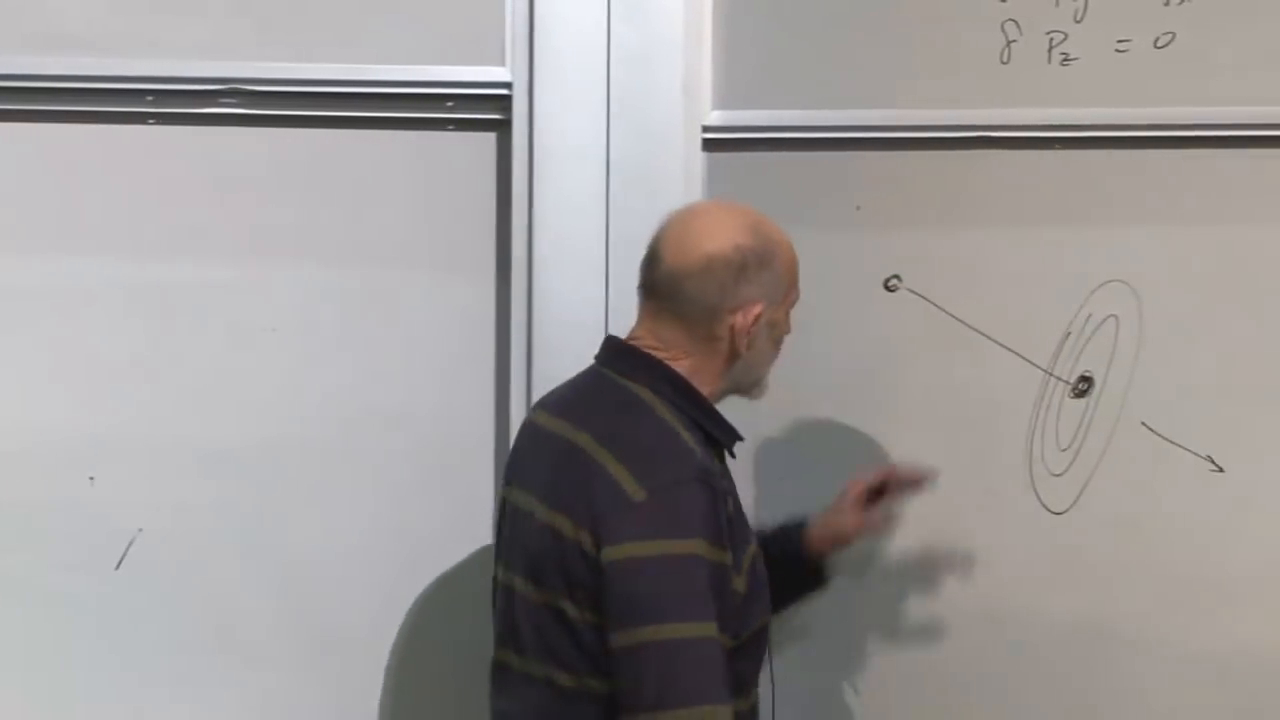
\includegraphics[width=0.82\textwidth]{lecture_08_figure_03.png}\caption{\(L_z\)와 좌표의 괄호: 괄호가 \((x,y,z)\)의 무한소 회전을 재현한다.}\lectureframe{00:38:41}\end{figure}

운동량도 벡터이므로 같은 계산을 하면 다음을 얻는다. \begin{equation}
  \begin{aligned}
    \{p_x,L_z\}&=-p_y,\\
    \{p_y,L_z\}&=p_x,\\
    \{p_z,L_z\}&=0.
  \end{aligned}
  \label{eq:l8-momentum-rotation-brackets}
\end{equation}

\begin{figure}[htbp]\centering
  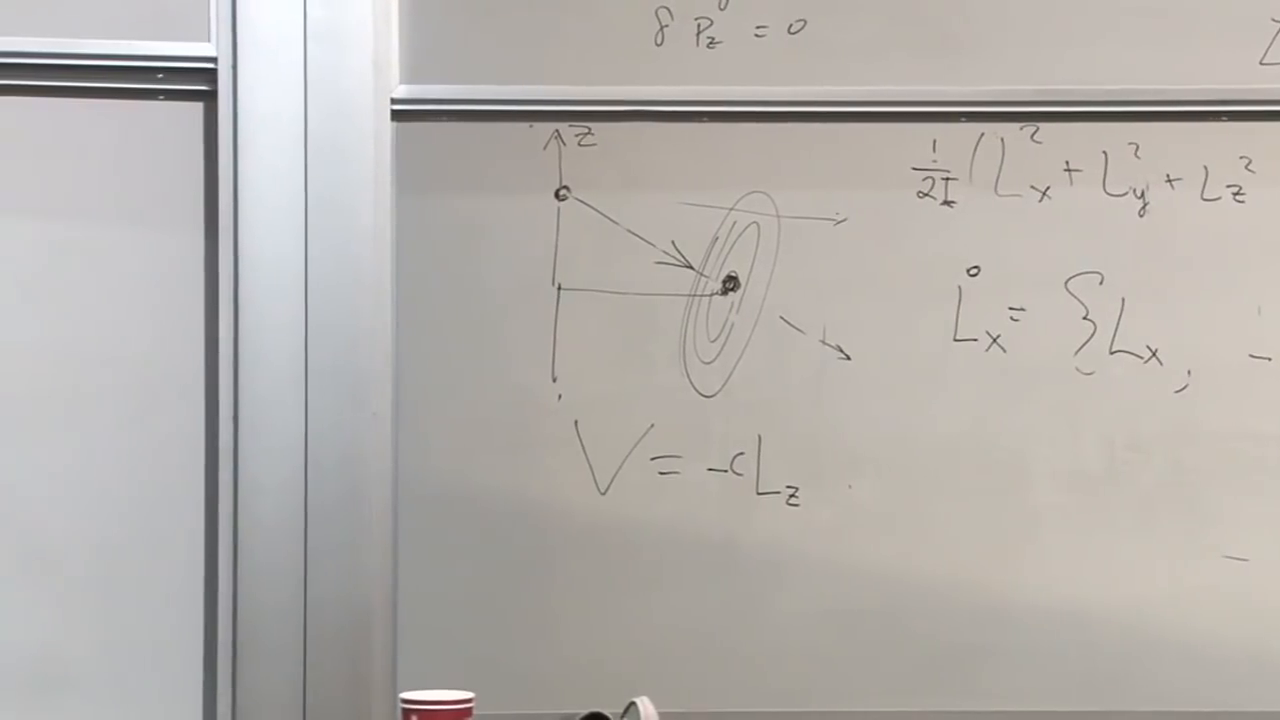
\includegraphics[width=0.82\textwidth]{lecture_08_figure_04.png}\caption{회전 생성자 \(L_z\)에 의해 위치와 운동량은 같은 벡터 형태로 변환된다.}\lectureframe{00:42:08}\end{figure}

따라서 일반적인 해밀턴 형식의 진술은 다음과 같다. \begin{equation}
  \boxed{\delta_G A=\epsilon\{A,G\}.}
  \label{eq:l8-generator-rule}
\end{equation} 위상 공간의 모든 함수 \(G\)는 이러한 무한소 정준 변환을 정의한다. \(G=L_z\)이면 회전이다. \(G=H\)이면 시간의 작은 변화이다.

\begin{classroomqa}\audiencequestion{강의에서는 어떤 때는 계를 회전시킨다고 하고, 어떤 때는 좌표를 회전시킨다고 합니다. 괄호 방정식에서는 어떤 규약을 쓰나요? \lecturetimestamp{00:28:22--00:29:35}} \lecturerresponse{식 ~\eqref{eq:l8-z-rotation}이 규약을 정한다. 이는 무한소 능동 회전 \((x,y)\mapsto(x-\epsilon y,y+\epsilon x)\)이다. 좌표축을 수동적으로 회전시키면 부호가 반대가 된다. 규약을 정하고 나면 괄호 공식은 모호하지 않다.}\end{classroomqa}

\section{운동량은 병진을 생성한다}

한 좌표 방향의 병진은 \begin{equation}
  \delta q=\epsilon.
  \label{eq:l8-q-translation}
\end{equation}이다. 여기서 식 ~\eqref{eq:l8-noether-variation}의 \(F(q)=1\)이므로, 이에 대응하는 보존량은 \(p\)이다. 생성자라는 주장은 다음을 예측한다. \begin{equation}
  \{f(q),p\}=\frac{df}{dq}.
  \label{eq:l8-translation-derivative}
\end{equation} 강의에서는 먼저 거듭제곱에 대해 귀납법으로 이를 증명한다. 기초 단계는 \(\{q,p\}=1\)이다. 다음을 가정하자. \begin{equation}
  \{q^{n-1},p\}=(n-1)q^{n-2}.
  \label{eq:l8-induction-hypothesis}
\end{equation} 그러면 곱의 법칙에 따라 \begin{align}
  \{q^n,p\}
  &=\{q\,q^{n-1},p\}\\
  &=q\{q^{n-1},p\}+\{q,p\}q^{n-1}\\
  &=(n-1)q^{n-1}+q^{n-1}\\
  &=nq^{n-1}.
  \label{eq:l8-power-translation}
\end{align} 선형성을 이용하면 이 결과를 다항식과 수렴하는 멱급수 표현으로 확장할 수 있다. 더 직접적으로는 괄호의 정의에서 미분 가능한 모든 \(f(q)\)에 대해 식 ~\eqref{eq:l8-translation-derivative}이 성립함을 알 수 있다. \begin{equation}
  \{f(q),p\}
  =
  \frac{\partial f}{\partial q}
  \frac{\partial p}{\partial p}
  =f'(q).
\end{equation}

\begin{figure}[htbp]\centering
  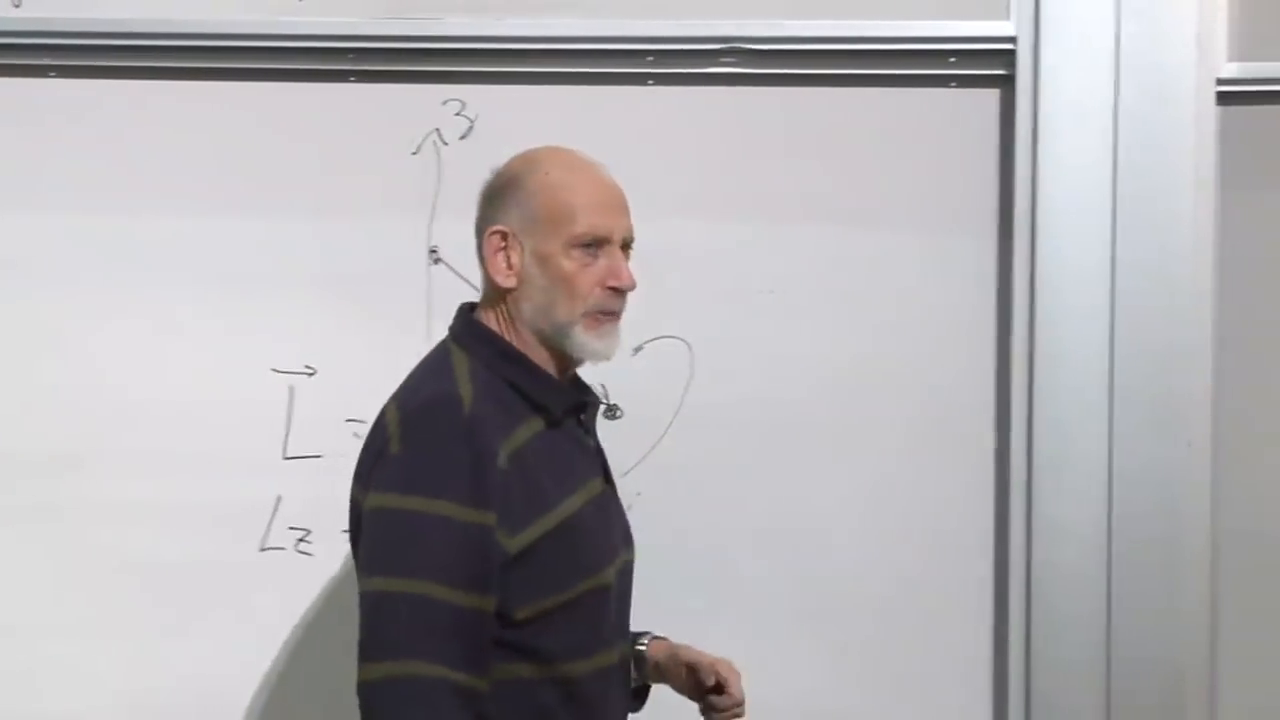
\includegraphics[width=0.82\textwidth]{lecture_08_figure_05.png}\caption{귀납법으로 얻은 병진 결과: \(\{F(q),p\}=dF/dq\).}\lectureframe{00:53:18}\end{figure}

이제 하나의 생각이 세 가지 형태로 나타남을 보았다. \begin{center}\begin{tabular}{@{}>{\raggedright\arraybackslash}p{0.37\textwidth}
                      >{\raggedright\arraybackslash}p{0.55\textwidth}@{}}\toprule
    생성자와 변환 &무한소 작용\\ \midrule
    \(H\)&\(\delta_tA=\epsilon\{A,H\}\)\\ \(p_i\)&\(\delta A=\epsilon\{A,p_i\}\)\\ \(L_i\)&\(\delta A=\epsilon\{A,L_i\}\)\\ \bottomrule
  \end{tabular}\end{center}연속 대칭에 대응하는 보존량은 그 대칭의 생성자이기도 하다.

\section{하나의 괄호, 두 가지 해석}

\(G(q,p)\)를 생성자 후보라고 하자. 이것이 보존되고 시간에 명시적으로 의존하지 않는다면, \begin{equation}
  \dot G=\{G,H\}=0.
  \label{eq:l8-g-conserved}
\end{equation} 반대칭성에 따라 \begin{equation}
  \{H,G\}=0.
  \label{eq:l8-h-invariant}
\end{equation} 수학적으로 두 식은 동등하지만, 물리적 해석은 다르다. \begin{itemize}\item \(\{G,H\}=0\)은 \(G\)가 \(H\)에 의해 생성되는 시간 변화 중에 변하지 않는다는 뜻이다. \item \(\{H,G\}=0\)은 \(H\)가 \(G\)에 의해 생성되는 변환 중에 변하지 않는다는 뜻이다.\end{itemize} 첫 번째는 보존 법칙이고 두 번째는 해밀토니안의 대칭성이다. 뇌터의 연결은 하나의 0으로 압축되어 있다.

\begin{figure}[htbp]\centering
  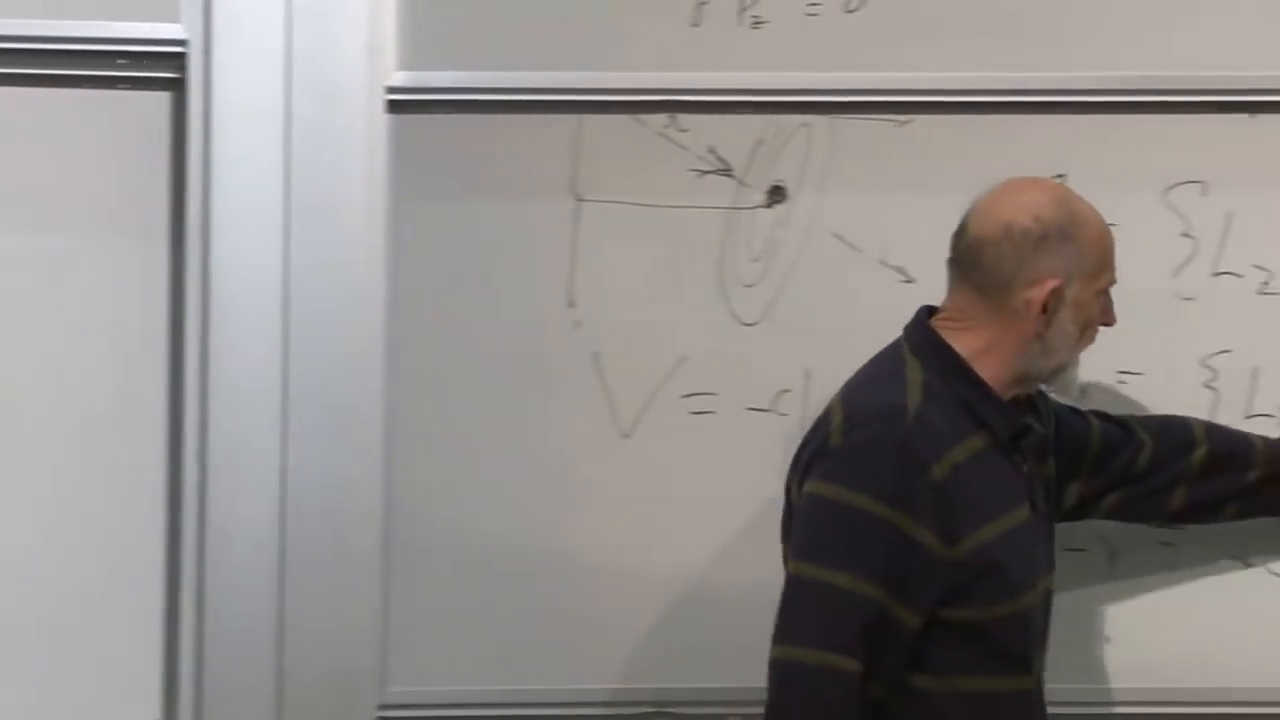
\includegraphics[width=0.82\textwidth]{lecture_08_figure_06.png}\caption{같은 영 괄호를 두 순서로 쓴 표현: \(G\)의 보존과 \(G\)가 생성하는 변환에 대한 \(H\)의 불변성.}\lectureframe{01:03:05}\end{figure}

\begin{classroomqa}\audiencequestion{보존량을 알고 있다면 그에 대응하는 대칭을 언제나 복원할 수 있나요? \lecturetimestamp{01:01:42--01:02:15}} \lecturerresponse{이 해밀턴 형식 안에서는 가능하다. 위상 공간 변수마다 \(G\)와 괄호를 취하면 된다. 그 결과인 모음 \(\delta_GA=\epsilon\{A,G\}\)은 변수들이 어떻게 변환되는지를 알려 준다. 예를 들어 \(L_z\)와의 괄호는 그 해석을 미리 몰랐더라도 회전을 드러낸다. 더 발전된 맥락에서는 전역적·경계 관련 미묘한 문제가 생길 수 있지만, 여기서는 국소적인 무한소 진술을 사용한다.}\end{classroomqa}

\begin{classroomqa}\audiencequestion{이 괄호 방정식은 보존 법칙을 일으키는 물리적 운동을 알려 주나요? \lecturetimestamp{00:56:01--00:58:13}} \lecturerresponse{아니다. 이 식들은 대칭 변환을 특정할 뿐 실제 궤적을 나타내지는 않는다. \(L_z\)의 보존은 회전 대칭을 뜻하지만, 입자가 원운동을 한다는 뜻은 아니다. 실제 시간 변화는 \(H\)에 의해 생성된다. 다른 생성자와의 괄호는 위상 공간에서 또 다른 변환 방향을 나타낸다.}\end{classroomqa}

\begin{classroomqa}\audiencequestion{보존을 미리 가정하지 않는 일반적인 변환 진술이 있나요? \lecturetimestamp{01:02:40--01:04:45}} \lecturerresponse{있다. 식 ~\eqref{eq:l8-generator-rule}은 함수 \(G\)마다 보존 여부와 관계없이 무한소 변환을 정의한다. 해밀토니안이 불변일 때만 대칭이 된다. 즉 \(\{H,G\}=0\)이다. 이를 반대 순서로 읽으면 \(G\)가 보존된다는 뜻이기도 하다.}\end{classroomqa}

\section{각운동량 대수}

다음 계산을 통해 회전 문제마다 입자 좌표를 계속 끌고 다니지 않아도 된다. 다음에서 시작하자. \[
  L_x=yp_z-zp_y,\qquad
  L_z=xp_y-yp_x.
\] \(\{L_x,L_z\}\)에서는 지수들이 정준쌍을 이루지 않으므로 대부분의 교차항이 사라진다. 남는 수축항을 계산하면 다음과 같다. \begin{align}
  \{L_x,L_z\}
  &=\{yp_z-zp_y,xp_y-yp_x\}\\
  &=xp_z-zp_x\\
  &=-L_y.
  \label{eq:l8-lx-lz}
\end{align} 순서를 바꾸면 음의 부호가 사라진다. 좌표를 순환적으로 바꾸면 다음을 얻는다. \begin{equation}
  \boxed{\begin{aligned}
    \{L_x,L_y\}&=L_z,\\
    \{L_y,L_z\}&=L_x,\\
    \{L_z,L_x\}&=L_y.
  \end{aligned}}
  \label{eq:l8-angular-algebra}
\end{equation} 지표 표기법으로는 다음과 같다. \begin{equation}
  \{L_i,L_j\}=\varepsilon_{ijk}L_k.
  \label{eq:l8-angular-algebra-index}
\end{equation}

\begin{figure}[htbp]\centering
  \includegraphics[width=0.82\textwidth]{lecture_08_figure_07.png}\caption{각운동량 세 성분의 순환 푸아송 괄호 대수.}\lectureframe{01:10:52}\end{figure}

이 결과는 미리 예측할 수도 있었다. \(\boldsymbol L\)는 벡터이므로, 그 \(x\) 성분과 \(L_z\)의 괄호는 \(z\)축 회전 아래 그 성분의 무한소 변화를 주어야 한다. 그 값은 \(-L_y\)이다. 명시적인 계산은 이 기하학적 논증을 확인해 준다. 이 방정식들은 양자 각운동량 교환 관계의 고전적 선구이기도 하다.

\section{빠르게 회전하는 자이로스코프}

응용으로 자이로스코프를 생각해 보자. 받침점에서 고정된 거리 \(R\)에 중심이 있는 고속 회전 플라이휠이다. 받침점에서 바퀴 중심을 향하는 벡터를 \(\boldsymbol r\)라 하자. 플라이휠은 축 둘레로 매우 빠르게 회전하므로, 지배적인 각운동량은 그 방향과 계속 나란하다. 강의에서 사용한 근사에서는 \begin{equation}
  \boldsymbol L=\ell\,\boldsymbol r,
  \qquad
  L_z=\ell z,
  \label{eq:l8-L-parallel-r}
\end{equation}이며, 여기서 \(\ell=L/R\)는 상수로 취급한다. 세차 운동이나 축의 운동에 관련된 더 작은 각운동량은 우선 무시한다.

\begin{figure}[htbp]\centering
  \begin{tikzpicture}[scale=0.95,>=Latex]
    \coordinate (P) at (0,3.2);
    \coordinate (C) at (3.7,1.55);
    \draw[->] (0,-0.2) -- (0,4.35) node[above] {\(z\)};
    \fill (P) circle (1.7pt) node[left] {pivot};
    \draw[very thick,->] (P) -- (C)
      node[midway,above right] {\(\boldsymbol r\parallel\boldsymbol L\)};
    \fill (C) circle (1.7pt);
    \draw[dashed] (P) -- (0,1.55);
    \draw[dashed] (0,1.55) -- (C);
    \node[left] at (0,1.55) {\(z\)};
    \begin{scope}[shift={(C)},rotate=-24]
      \draw[very thick] (0,0) ellipse (0.65 and 1.35);
      \draw[thick] (0,0) ellipse (0.42 and 0.9);
    \end{scope}
    \draw[->,thick] (2.15,2.85)
      arc[start angle=140,end angle=35,radius=1.65];
  \end{tikzpicture}\caption{빠른 자이로스코프 근사. 받침점과 중심 사이의 거리는 고정되어 있고, 지배적인 스핀 각운동량은 축 및 \(\boldsymbol r\)와 나란하게 유지된다.}\end{figure}

\begin{figure}[htbp]\centering
  \includegraphics[width=0.82\textwidth]{lecture_08_figure_08.png}\caption{플라이휠, \(H_{\rm rot}=L^2/(2I)\), 그리고 토크가 없을 때 \(\boldsymbol L\)가 보존됨을 보이는 소거를 칠판에 스케치한 그림.}\lectureframe{01:18:54}\end{figure}

\subsection{중력이 없을 때: 모든 성분이 고정되는 이유}

단순화한 축대칭 회전자의 경우, \begin{equation}
  H_{\mathrm{rot}}
  =\frac{1}{2I}
  \left(L_x^2+L_y^2+L_z^2\right)
  =\frac{L^2}{2I}.
  \label{eq:l8-rotational-hamiltonian}
\end{equation} 계수는 \(I/2\)이 아니라 \(1/(2I)\)이다. 칠판에서는 이 부분을 잘못 썼다가 바로잡는다. 식 ~\eqref{eq:l8-angular-algebra}을 사용하면, \begin{align}
  \dot L_x
  &=\{L_x,H_{\mathrm{rot}}\}\\
  &=\frac{1}{2I}\left(
    2L_y\{L_x,L_y\}
    +2L_z\{L_x,L_z\}
  \right)\\
  &=\frac{1}{I}\left(L_yL_z-L_zL_y\right)=0.
  \label{eq:l8-free-lx}
\end{align} 순환적으로 다음도 성립한다. \begin{equation}
  \dot L_x=\dot L_y=\dot L_z=0.
  \label{eq:l8-free-angular-momentum}
\end{equation} 스칼라 \(L^2\)는 각 성분 \(L_i\)과의 괄호가 0이다. 이 대수의 용어로는 카시미르이다. 따라서 토크가 없는 자이로스코프는 각운동량의 크기와 방향을 모두 유지한다.

\begin{classroomqa}\audiencequestion{여기서 관성 모멘트는 그냥 수 하나인가요? \lecturetimestamp{01:14:23--01:15:05}} \lecturerresponse{이 축약 모형에서는 그렇다. 관성 모멘트는 회전축에 대한 바퀴의 질량 분포를 나타낸다. 일반적인 강체에는 관성 모멘트 텐서가 있으며, 주축에서 회전 해밀토니안은 \(\sum_i L_i^2/(2I_i)\)이다. 이 강의에서는 완전한 강체 동역학을 전개하기보다 푸아송 괄호 방법을 보여 주려는 것이 목적이므로 더 단순한 고속 대칭 회전자를 택한다.}\end{classroomqa}

\subsection{중력과 퍼텐셜의 부호}

수직 좌표 \(z\)를 위쪽이 양의 방향이 되도록 잡고 받침점을 원점에 두자. 바퀴 중심의 중력 퍼텐셜 에너지는 \begin{equation}
  V=Mgz.
  \label{eq:l8-mgz}
\end{equation}이다. \(L_z=\ell z\)이므로, \begin{equation}
  V=cL_z,
  \qquad
  c=\frac{Mg}{\ell}=\frac{MgR}{L}.
  \label{eq:l8-potential-lz}
\end{equation}이다. 여기서 \(c>0\)은 \(\boldsymbol L\)가 \(\boldsymbol r\)와 평행하도록 정했을 때 성립한다. 플라이휠이 반대 방향으로 회전하면 \(\boldsymbol L\)와 \(\boldsymbol r\) 사이의 부호 있는 관계가 반전되며, 이에 따라 세차 각주파수의 부호도 바뀐다.

\begin{figure}[htbp]\centering
  \includegraphics[width=0.82\textwidth]{lecture_08_figure_09.png}\caption{\(\boldsymbol L=\ell\boldsymbol r\)와 \(L_z=\ell z\)에 해당하는 고정 길이 기하.}\lectureframe{01:25:38}\end{figure}

\begin{figure}[htbp]\centering
  \includegraphics[width=0.82\textwidth]{lecture_08_figure_10.png}\caption{칠판의 중간 단계에는 \(V=-cL_z\)가 나타난다. 나중에 \(z\)를 위쪽으로 정한 뒤 부호를 바로잡는다. \(\boldsymbol L=\ell\boldsymbol r\)와 \(\ell>0\)을 사용하면 일관된 결과는 \(V=+cL_z\)이다.}\lectureframe{01:22:43}\end{figure}

\begin{classroomqa}\audiencequestion{높이를 각운동량의 한 성분으로 바꾸어도 되는 이유는 무엇인가요? 비스듬한 선은 축인가요, 위치벡터인가요? \lecturetimestamp{01:22:20--01:25:43}} \lecturerresponse{비스듬한 선은 고정된 받침점에서 바퀴 중심까지의 벡터인 \(\boldsymbol r\)로 표시하는 것이 가장 적절하다. 실제 축이 그 방향을 따라 놓일 수는 있지만, 계산에서 사용하는 관계는 빠른 스핀 근사 \(\boldsymbol L=\ell\boldsymbol r\)이다. 따라서 두 벡터의 \(z\) 성분은 서로 비례한다. 실시간 강의에서는 이 구분을 확정하기 전에 표기를 몇 차례 바꾼다.}\end{classroomqa}

\begin{classroomqa}\audiencequestion{어떤 가정 아래서 \(\ell\)가 상수인가요? 바퀴 중심이 반지름 방향으로 미끄러질 수 있다면 무엇이 성립하지 않나요? \lecturetimestamp{01:25:43--01:26:38,\allowbreak\ 01:34:22--01:35:00}} \lecturerresponse{지배적인 스핀이 느린 운동에 따르는 각운동량보다 훨씬 크고, 받침점과 중심 사이의 거리가 고정되어 있다고 가정한다. 그러면 스핀의 크기는 거의 변하지 않고 \(\boldsymbol L\)는 \(\boldsymbol r\)와 함께 회전한다. 중심이 반지름 방향으로 미끄러질 수 있다면 \(z\)는 더 이상 하나의 상수 계수를 두고 \(L_z\)에 비례하지 않으므로, 축약 해밀토니안 \(V=cL_z\)으로는 운동을 기술할 수 없다.}\end{classroomqa}

\begin{classroomqa}\audiencequestion{칠판에 처음에는 음의 부호가 나오고 나중에는 양의 부호가 나오는 이유는 무엇인가요? 스핀 방향이 중요한가요? \lecturetimestamp{01:27:13--01:28:15,\allowbreak\ 01:33:09--01:33:21}} \lecturerresponse{처음의 부호는 칠판에 쓰는 도중의 오류와 정해지지 않은 축 규약이 섞인 결과다. \(z\)를 위쪽으로 정의하면 \(V=Mgz\)는 높이가 높아질수록 증가한다. \(\boldsymbol L=\ell\boldsymbol r\)와 \(\ell>0\)라면 \(V=+cL_z\)이다. 스핀을 반대로 하면 부호 있는 비례 관계와 세차 방향이 반전되지만, 임의로 부호를 선택해도 된다는 뜻은 아니다.}\end{classroomqa}

\subsection{세 개의 짧은 방정식으로 세차 운동 구하기}

축약된 전체 해밀토니안은 다음과 같다. \begin{equation}
  H=
  \frac{1}{2I}\left(L_x^2+L_y^2+L_z^2\right)+cL_z.
  \label{eq:l8-full-gyro-hamiltonian}
\end{equation} \(L^2\)는 모든 \(L_i\)와의 괄호가 0임을 이미 보였다. 따라서 선형 항만 기여한다. \begin{align}
  \dot L_z&=\{L_z,H\}=0,\\
  \dot L_x&=\{L_x,H\}=c\{L_x,L_z\}=-cL_y,\\
  \dot L_y&=\{L_y,H\}=c\{L_y,L_z\}=cL_x.
  \label{eq:l8-precession-equations}
\end{align}

\begin{figure}[htbp]\centering
  \includegraphics[width=0.82\textwidth]{lecture_08_figure_11.png}\caption{최종 성분 방정식: \(L_z\)는 일정하고 \(L_x\)와 \(L_y\)는 서로 변환되며 회전한다.}\lectureframe{01:30:35}\end{figure}

수직 성분과 수평 성분의 크기는 일정하다. \begin{equation}
  \frac{d}{dt}(L_x^2+L_y^2)
  =2L_x(-cL_y)+2L_y(cL_x)=0.
\end{equation} 수평 성분을 결합하면, \begin{equation}
  L_+=L_x+iL_y,
  \qquad
  \dot L_+=icL_+,
\end{equation} 따라서 \begin{equation}
  L_+(t)=L_+(0)e^{ict}.
  \label{eq:l8-precession-solution}
\end{equation} 각운동량 벡터는 수직축 둘레로 각속력 \(|c|=MgR/L\)로 세차한다. 이 이상화된 정상 운동에서는 기울기가 일정하게 유지된다.

\begin{classroomqa}\audiencequestion{세차 방정식을 쓸 때 회전 에너지 항을 무시했나요? \lecturetimestamp{01:35:01--01:35:49}} \lecturerresponse{아니다. 식 ~\eqref{eq:l8-full-gyro-hamiltonian}처럼 전체 해밀토니안에 포함된다. 다만 \(\dot L_i\)에 기여하지 않을 뿐이다. \(\{L_i,L^2\}=0\)이기 때문인데, 이는 토크가 없는 경우의 계산에서 이미 증명한 소거이다. 학생의 질문 덕분에 암묵적이었던 이 단계가 명시되었다.}\end{classroomqa}

\begin{classroomqa}\audiencequestion{균일 세차는 평형 상태인가요? 작은 충격을 주면 어떻게 되나요? \lecturetimestamp{01:32:38--01:33:08}} \lecturerresponse{정적인 평형 상태라기보다 정상 운동 또는 정상 상태의 운동이라고 부르는 편이 정확하다. 작은 충격을 주면 일반적으로 장동, 즉 기울기 각도의 진동이 더해진다. 매우 빠르게 회전하는 바퀴에서는 그 진동이 작으므로 축약된 설명에서는 거의 균일한 세차만 고려한다.}\end{classroomqa}

\begin{classroomqa}\audiencequestion{세차 운동에는 지지대나 실제 축이 필요한가요? \lecturetimestamp{01:31:49--01:32:38,\allowbreak\ 01:33:49--01:35:00}} \lecturerresponse{이 역학 모형에서는 받침점과 중심 사이의 거리가 고정되어 있다고 가정하므로, 어떤 구속력이 지지 역할을 한다. 더 일반적인 대수적 결과는 적용 범위가 넓다. 각운동량의 한 성분에 선형인 해밀토니안 항이 있으면 언제나 같은 괄호 대수로 세차 운동을 얻는다. 각운동량의 미시적 근원이 실제 축에 달린 바퀴일 필요는 없다.}\end{classroomqa}

\begin{classroomqa}\audiencequestion{이것은 자기장 속 전자 스핀이나 핵스핀의 세차 운동, 또는 행성 궤도의 세차 운동과 같은 현상인가요? \lecturetimestamp{01:35:50--01:37:00}} \lecturerresponse{자기장과 결합한 자기 모멘트는 스핀 성분에 선형인 해밀토니안을 가지므로 같은 각운동량 대수를 따른다. 핵스핀의 세차 운동은 핵자기공명에 쓰인다. 행성 궤도 근일점의 세차는 \emph{세차}라는 말을 공유할 뿐 다른 현상이며, 같은 계산이 아니다.}\end{classroomqa}

\begin{classroomqa}\audiencequestion{옆으로 장착된 자이로스코프는 본질적으로 팽이와 같은 물체인가요? \lecturetimestamp{01:37:02--01:37:23}} \lecturerresponse{그렇다. 차이는 주로 기하학적 표현에 있다. 회전축이 지지대에서 옆으로 뻗어 있을 때는 보통 자이로스코프라 하고, 거의 수직일 때는 팽이라고 한다. 각운동량과 토크의 구조는 같다.}\end{classroomqa}

\section{계산을 통해 얻은 것}

오일러각을 도입하지 않았고 바퀴의 모든 부분에 대한 좌표를 추적하지도 않았다. \[
  \{L_i,L_j\}=\varepsilon_{ijk}L_k
\]을 알고 나면 관심 있는 변수들의 방정식을 바로 얻을 수 있다. 이것이 보여 주려는 힘이다. 조화진동자에서는 푸아송 괄호가 익숙한 동역학을 재현할 수 있음을 보았다. 각운동량은 푸아송 괄호가 그 이상의 일을 한다는 점을 보여 주었다. \begin{itemize}\item 보존량은 그에 대응하는 무한소 대칭을 생성한다. \item \(G\)의 보존과 \(H\)의 불변성은 \(\{G,H\}=0\)의 두 가지 해석이다. \item 관측량의 대수는 그 자체 안에서 닫힐 수 있어 미시적 좌표로 되돌아가지 않고도 동역학을 풀 수 있다. \item 각운동량 성분 하나에 선형인 해밀토니안은 그 축 둘레의 세차 운동을 일으킨다.\end{itemize}강의는 일반적인 강체에 대한 완전한 오일러 방정식을 다루기 전에 끝난다. 그보다 좁은 결론은 이미 완결되었다. 적절한 생성자와 그 푸아송 대수는 대칭과 운동을 놀라울 만큼 간결하게 드러낸다.